\section{Evaluation}
This section answers the following research questions:
\begin{itemize}[leftmargin=12pt, topsep=0pt]
    \item \textbf{RQ1}: How effective is \name in anomaly detection?
    \item \textbf{RQ2}: How effective is \name in root cause localization?
    \item \textbf{RQ3}: How much does each data source contribute?
\end{itemize}

\subsection{Data Collection}\label{sec:data}
Since existing data collections of microservice systems~\cite{AiopsChallenge20, TraceData20} contain traces only, we deploy two benchmark microservice systems and generate requests to collect multi-source data, including logs, KPIs, and traces.
Afterward, we inject typical faults to simulate real-world anomalies.
To our best knowledge, it is the first triple-source data collection 
 with injected faults in the context of microservices.

\subsubsection{Benchmark microservice systems}
We first deploy two open-source microservice benchmarks: TrainTicket~\cite{TrainTicket} (TT) and SocialNetwork~\cite{SocialNetwork} (SN).
TT provides a railway ticketing service where users can check, book, and pay for train tickets. It is widely used in previous works~\cite{MEPFL, TraceAnomaly} with 41 microservices actively interacting with each other, and 27 of them are business-related.
SN implements a broadcast-style social networking site. Users can create, read, favorite, and repost posts. In this system, 21 microservices communicate with each other via Thrift RPCs~\cite{Thrift}.
SN has 21 microservices, 14 of which are related to business logic. 
 
We construct a distributed testbed to deploy the two systems running in Docker containers and develop two request simulators to simulate valid user requests.
A series of open-source monitoring tools are deployed for data collection.
Microservice instances send causally-related traces to a collector Jaeger~\cite{Jaeger}.
We employ cAdvisor~\cite{cAdvisor} and Prometheus~\cite{Prometheus} to monitor the KPIs per second of each microservice.
The KPIs are stored in an instance of InfluxDB~\cite{Influxdb}, including ``CPU system usage'', ``CPU total usage'', ``CPU user usage'', ``memory usage'', the amount of ``working set memory'', ``rx bytes'' (received bytes), and ``tx bytes'' (transmitted bytes). 
We also utilize Elasticsearch~\cite{Elasticsearch}, Fluentd~\cite{Fluentd}, and Kibana~\cite{Kibana} to collect, aggregate, and store logs, respectively.

\subsubsection{Fault Injection}
\name can troubleshoot anomalies that manifest themselves in performance degradations (logs and KPIs) or latency deviations (traces). Referring to previous studies~\cite{MicroRank, AutoMAP, DyCause}, we inject three typical types of faults via Chaosblade~\cite{Chaosblade}. 
Specifically, we simulate CPU exhaustion by putting a hog to consume CPU resource heavily. 
To simulate a network jam, we delay the network packets of a microservice instance. 
We also randomly drop network packets to simulate stochastic packet loss that frequently occurs when excessive data packets flood a network.

We generate 0.2$\sim$0.5 and 2$\sim$3 requests per second for TT and SN at a uniform rate, respectively.
Before fault injection, we collect normal data under a fault-free setting for 7 hours for TT and 1.2 hours for SN.
Then, we set each fault duration to 10 mins (with a 2-min interval between two injections) for TT, while the fault duration is 2 mins and SN's interval is half a minute. 
Each fault is injected into one microservice once.
In total, we conduct 162 and 72 injection operations in TT and SN, respectively.
Such different setups are attributed to the different processing capacities of the two systems, i.e., TT usually takes more time to process a request than SN.

In this way, we collect two datasets (\A and \B) with 48,296 and 126,384 traces, respectively. Data produced in different periods are divided into training (60\%) data and testing (40\%) data, respectively. The data divisions share similar distributions in abnormal/normal ratios and root causes.

\subsection{Baselines} 
We compare \name with previous approaches and derived methods integrating multi-source data. As our task is relatively novel by incorporating more information than existing single-source data-based studies, simply comparing our model with previous approaches seems a bit unfair.

\subsubsection{Advanced baselines} 
In terms of anomaly detection, we consider two state-of-the-art baselines.
TraceAnomaly~\cite{TraceAnomaly} uses a variational auto-encoder (VAE) to discover abnormal invocations. 
MultimodalTrace~\cite{MMTrace} extracts operation sequences and latency time series from traces and uses a multi-modal Long Short-term Memory (LSTM) network to model the temporal features.
For root cause localization, we compare \name with five trace-based baselines: TBAC~\cite{TBAC}, NetMedic~\cite{NetMedic}, MonitorRank~\cite{MonitorRank}, CloudRanger~\cite{CloudRanger}, and DyCause~\cite{DyCause}.
As far as we know, no root cause localizers for microservices rely on multi-modal data. 

These methods use statistical models or heuristic methods to locate the root cause. For example, TBAC, MonitorRank, and DyCause applied the Pearson correlation coefficient, and MonitorRank and DyCause also leveraged Random Walk.
We implement these baselines referring to the codes provided by the original papers~\cite{TraceAnomaly, DyCause, MicroRank}. For the papers without open-source codes, we carefully follow the papers and refer to the baseline implementation released by~\cite{DyCause}.

\subsubsection{Derived multi-source baselines} \label{sec:setup:derived}
We also derive four multi-source data-based methods for further comparison.
Inspired by~\cite{MMTrace}, we transform all data sources into time series and use learning-based algorithms for status inference. 
Specifically, logs are represented by event occurrence sequences; traces are denoted by latency time series; KPIs are natural time series.
Since previous studies are mainly machine learning-based, we train practical machine learning methods, i.e., Random Forest (RF) and Support Vector Machine (SVM), on the multi-source time series.
We derive MS-RF-AD and MS-SVM-AD for anomaly detection as well as MS-RF-RCL and MS-SVM-RCL for root cause localization.
We also derive two methods (MS-LSTM and MS-DCC) that employ deep learning techniques, i.e., LSTM and 1D DCC, to extract representations from multi-modal time series.
The learned representations are fed into the module of joint detection and localization, which is described in~\ref{sec:method:output}.

\subsection{Implementation}
The experiments are conducted on a Linux server with an NVIDIA GeForce GTX 1080 GPU via Python 3.7. 
As for the hyper-parameters, the hidden size of all fully-connected layers is 64, and every DCC layer shares the same filter number of 64 with a kernel size of three. The GAT's hidden size and the fusion dimension (i.e., $2E$) are 128.
We use a 4-head mechanism of GAT's attention layer, and the layer number of all modalities' models is only one for speeding up.
Moreover, Batch Normalization~\cite{BatchNorm} is added after DCCs to mitigate overfitting.
We train \name using the Adam~\cite{Adam} optimizer with an initial learning rate of 0.001, a batch size of 256, and an epoch number of 50.
All the collected data and our code are released for replication.

\subsection{Evaluation Measurements}
The anomaly detection challenge is modeled in a binary classification manner, so we apply the widely-used binary classification measurements to gauge the performance of models:
Recall (\textit{Rec})$=\frac{TP}{TP+FN}$, Precision (\textit{Pre})$=\frac{TP}{TP+FP}$, F1-score (\textit{F1})$=\frac{2 \cdot Pre \cdot Rec}{Pre+Rec}$,
where $TP$ is the number of discovered abnormal samples; $FN$ and $FP$ are defined in~\cref{sec:study:detection}.

For root cause localization, we introduce the Hit Rate of top-k (\textit{HR@k}) and Normalized Discounted Cumulative Gain of top-k (\textit{NDCG@k}) for localizer evaluation. Herein, we set $k=1,3,5$.
\textit{HR@k}$=\frac{1}{N} \sum_{i=1}^N(s_i^t \in S^{p}_{i, [1:k]})$ calculates the overall probability of the culprit microservice within the top-k predicted candidates $S^{p}_{i, [1:k]}$, where $s_i^t$ is the ground-truth root cause for the $i$-th observation window, and $N$ is the number of samples to be tested. 
\textit{NDCG@k}$=\frac{1}{N} \sum_{i=1}^N (\sum_{j=1}^M \frac{p_j}{\log_2(j+1)})$ measures the ranking quality, where $p_j$ is the predicted probability of the $j$-th microservice, and $M$ is the number of microservices. 
\textit{NDCG@1} is left out because it is the same with \textit{HR@1} in our scenario.
The two evaluation metrics measure how easily engineers find the culprit microservice. \textit{HR@k} directly measures how likely the root cause will be found within $k$ checks. \textit{NDCG@k} measures to what extent the root cause appears higher up in the ranked candidate list.
Thus, the higher the above measurements, the better. 

\subsection{\textbf{RQ1}: Effectiveness in Anomaly Detection}
\begin{table}[htbp]
\small
\centering
\vspace{-0.15in}
\caption{Performance Comparison for Anomaly Detection}
\begin{adjustbox}{max width=\columnwidth}
\begin{tabular}{l*{7}{c}}
\toprule
\multirow{2}*{\centering \textbf{Approaches}} & \multicolumn{3}{c}{\A} & \multicolumn{3}{c}{\B}\\
\cmidrule(lr){2-4}\cmidrule(lr){5-8}
&\textit{F1}&\textit{Rec}&\textit{Pre}&\textit{F1}&\textit{Rec} &\textit{Pre}\\
\cmidrule{1-8}\morecmidrules\cmidrule{1-8}
TraceAnomaly & 0.486 & 0.414 & 0.589 & 0.539 & 0.468 & 0.636 \\
MultimodalTrace & 0.608 & 0.576 & 0.644 & 0.676 & 0.632 & 0.726\\
\hdashline[2pt/5pt]
MS-RF-AD & 0.817 & 0.705 & 0.971 & 0.773 & 0.866 & 0.700 \\
MS-SVM-AD & 0.787 & 0.678 & 0.938 & 0.789 & 0.770 & 0.808\\
MS-LSTM & 0.967 & 0.997 & 0.940 & 0.948 & 0.959 & 0.937 \\
MS-DCC & 0.965 & 0.993 & 0.938  & 0.948 & 0.962 & 0.934 \\
\midrule
\textbf{\name} & \textbf{0.989} & \textbf{0.995} & \textbf{0.984} & \textbf{0.986} & \textbf{0.996} & \textbf{0.977}\\
%F1: 0.9875, 
\bottomrule
\end{tabular}
\end{adjustbox}
\label{tab:exp:detection}
\end{table}

Ground truths are based on the known injection operations, i.e., if a fault is injected, then the current observation window is abnormal; otherwise, it is normal. Table~\ref{tab:exp:detection} displays a comparison of anomaly detection, from which we draw three observations:

(1) \name outperforms all competitors significantly and achieves very high scores in \textit{F1} (0.988), \textit{Rec} (0.996), and \textit{Pre} (0.981), illustrating that \name generates very few missing anomalies or false alarms.
\name's excellence can be attributed to 1) \name applies modality-specific designs to model various sources of data as well as a multi-modal fusion to wrangle these modalities so that it can learn a distinguishable representation of the status; 2) \name learns dependencies between microservices to enable extraction of anomaly propagation to facilitate tracing back to the root cause.

(2) Generally, multi-source data-based approaches, including \name, perform much better than trace-relied baselines because they incorporate extra essential information (i.e., logs and KPIs) besides traces. 
The results align with our observations in~\cref{sec:study:multi-source} that logs and KPIs provide valuable clues about microservice anomalies, while traces cannot reveal all anomalies.
Trace-based methods can only detect anomalies yielding an enormous impact on invocations, so they ignore anomalies reflected by other data sources.

(3) Moreover, \name, MS-LSTM, and MS-DDC perform better than MS-SVM and MS-RF. 
The superiority of the former ones lies in applying deep learning and joint learning. 
Deep learning has demonstrated a powerful capacity in extracting features from complicated time series~\cite{TCNexp, DeepTSCreview, TSDMreview}. 
Joint learning allows capturing correlated knowledge across detection and localization to exploit commonalities across the two tasks.
These two mechanisms are beneficial to troubleshooting by enhancing representation learning.

In brief, \name is very effective in anomaly detection of microservice systems and improves \textit{F1} by 53.82\%$\sim$92.68\% compared to baselines and 3.13\%$\sim$25.32\% compared to derived methods. 
The detector is of tremendous assistance for next-stage root cause localization by reducing noisy labels inside the localizer's inputs.

\subsection{\textbf{RQ2}: Effectiveness in Root Cause Localization}
\begin{table*}[htbp]
\small
\centering
\caption{Performance Comparison for Root Cause Localization}
\begin{tabular}{l*{10}{c}}
\toprule
\multirow{2}*{\centering \textbf{Approaches}} & \multicolumn{5}{c}{\A} & \multicolumn{5}{c}{\B}\\
\cmidrule(lr){2-6}\cmidrule(lr){7-11}
&\textit{HR@1}&\textit{HR@3}&\textit{HR@5}&\textit{NDCG@3}&\textit{NDCG@5}&\textit{HR@1}&\textit{HR@3}&\textit{HR@5}&\textit{NDCG@3}&\textit{NDCG@5} \\
\cmidrule{1-11}\morecmidrules\cmidrule{1-11}
TBAC & 0.037 & 0.111 & 0.185 & 0.079 & 0.109 & 0.001 & 0.085 & 0.181 & 0.048 & 0.087 \\
NetMedic & 0.094 & 0.257 & 0.425 & 0.195 & 0.209 & 0.069 & 0.187 & 0.373 & 0.146 & 0.218 \\
MonitorRank & 0.086 & 0.199 & 0.331 & 0.142 & 0.196 & 0.068 & 0.118 & 0.221 & 0.095 & 0.137\\
CloudRanger & 0.101 & 0.306 & 0.509 & 0.218 & 0.301 & 0.122 & 0.382 & 0.629 & 0.269 & 0.370\\
DyCause & 0.231 & 0.615 & 0.808 & 0.448 & 0.607 & 0.273 & 0.636 & 0.727 & 0.301 & 0.353 \\
\hdashline[1pt/5pt]
MS-RF-RCL & 0.637 & 0.922 & \underline{0.970} & 0.807 & 0.827 &0.704 & \underline{0.908} & \underline{0.970} & 0.825 & \underline{0.851}\\
MS-SVM-RCL& 0.541 & 0.908 & 0.944 & 0.814 & 0.820 & 0.614 & 0.838 & \underline{0.955} & 0.741 & 0.790 \\
MS-LSTM & 0.756 & 0.930 & \underline{0.969}	& 0.859 & 0.877 & 0.757 & \underline{0.884} & \underline{0.907} & 0.834 & \underline{0.844}\\
MS-DCC & 0.767 & 0.938 & 0.972 & 0.870 & 0.882 & 0.789 & 0.968 & 0.985 & 0.898 & 0.905\\
\midrule 
\textbf{\name} & \textbf{0.990} & \textbf{0.992} & \textbf{0.993} & \textbf{0.994} & \textbf{0.994} & \textbf{0.974} & \textbf{0.988} & \textbf{0.991} & \textbf{0.982} & \textbf{0.983}\\
\bottomrule
\end{tabular}
\vspace{-0.1in}
\label{tab:exp:localization}
\end{table*}

To focus on comparing the effectiveness of root cause localization, we provide ground truths of anomaly existence for baselines herein.
In contrast, \name, MS-LSTM, and MS-DCC use the predicted results of their detectors as they are end-to-end approaches integrating the two tasks.
Table~\ref{tab:exp:localization} presents the root cause localization comparison, underpinning three observations:

(1) \name performs the best, taking all measurements into consideration, achieving \textit{HR@1} of 0.982, \textit{HR@5} of 0.990, and \textit{NDCG@5} of 0.989 on average.
With the incorporation of valuable logs and KPIs ignored by previous approaches, \name can depict the system status more accurately.
Trace-based approaches have difficulties in troubleshooting resource exhaustion-related anomalies or severe network-related anomalies that block inter-service communications resulting in few invocations.
Besides, \name enables eavesdropping across detection and localization via joint learning, which encourages full use of the shared knowledge to enhance status learning. 
\name also leverages powerful techniques to capture meaningful patterns from multi-modal data, including designs of modality-specific models and advanced GAT to exploit graph-structure dependencies. 
Moreover, \name achieves a much higher score in \textit{HR@1} than derived methods, while its superiority in \textit{HR@5} and \textit{NDCG@5} is not particularly prominent.
The reason is that \name learns the dependency-aware status besides intra-service behaviors, allowing to catch the anomaly origin by tracing anomaly propagation.
Other multi-modal approaches capture dependency-agnostic information, so they can pinpoint the scope of suspicious microservices effectively rather than directly deciding the culprit.

(2) Multi-modal approaches considerably outperform single-modal baselines, similar to the results in anomaly detection.
The superiority of multi-source derived methods is more evident since localization is a more complicated task than detection, so the advantage of incorporating diverse data sources to learn the complementarity is fully demonstrated.
This situation is more revealing in \A because TrainTicket responds more slowly, leading to sparse trace records, and trace-based models get into trouble when few invocations occur in the current observation window.
In contrast, derived approaches can accurately locate the culprit microservice in such a system since they leverage various information sources to obtain more clues.

(3) Considering multi-modal approaches, \name, MS-LSTM, and MS-DCC deliver better performance (measured by \textit{HR@1}) than MS-RF-RCL and MS-SVM-RCL.
The superiority of the former approaches can be attributed to the strong fitting ability of deep learning and the advantages brought by the joint learning mechanism.
However, MS-LSTM performs poorer in narrowing the suspicious scope, especially in \B (measured by \textit{HR@5} and \textit{NDCG@5}).
This may be because that LSTMs' training process is a lot more complicated than DCCs or simple machine learning techniques. The scale of \B is relatively small, so MS-LSTM cannot be thoroughly trained and capture the most meaningful features.

To sum up, the results demonstrate the effectiveness of \name in root cause localization. \name increases \textit{HR@1} by 290\%$\sim$5068\% than baselines and 26.93\%$\sim$66.16\% than derived methods.
Our approach shows effectiveness both in anomaly detection and root cause localization, suggesting its potential to automate labor-intensive troubleshooting.

\subsection{\textbf{RQ3}: Contributions of Different Data Sources}
We perform an ablation study to explore how different data sources contribute by conducting source-wise-agnostic experiments, so we derive the following variants:

\begin{itemize}[leftmargin=12pt, topsep=0pt]
    \item \name w/o $\mathcal{L}$: drops logs while inputs traces and KPIs by removing the log modeling module in \cref{sec:method:log}.
    \item \name w/o $\mathcal{M}$: drops KPIs while inputs traces and logs by removing the KPI modeling module in \cref{sec:method:KPI}.
    \item \name w/o $\mathcal{T}$: drops latency extracted from traces by removing the trace modeling module in \cref{sec:method:trace}.
    \item \name w/o $\mathcal{G}$: replaces GAT by an FC layer to learn dependency-agnostic representations.
\end{itemize}

\begin{table}[htb]
\small
\centering
\vspace{-0.1in}
\caption{Experimental Results of the Ablation Study}
\begin{adjustbox}{max width=\columnwidth}
\begin{tabular}{lcccccc}
\toprule
\multirow{2}*{\centering \textbf{Variants}} & \multicolumn{3}{c}{\A} & \multicolumn{3}{c}{\B}\\
\cmidrule(lr){2-4}\cmidrule(lr){5-7}
&\textit{HR@1}&\textit{HR@5}&\textit{F1}&\textit{HR@1}&\textit{HR@5}&\textit{F1}\\
\cmidrule{1-7}\morecmidrules\cmidrule{1-7}
\textbf{\name} & \textbf{0.990} & \textbf{0.993} & \textbf{0.989} & \textbf{0.974} & \textbf{0.991}& \textbf{0.986}\\
\midrule
{\name w/o $\mathcal{L}$} & 0.926 & 0.993 & 0.964 & 0.902 & 0.954 & 0.972\\
{\name w/o $\mathcal{M}$} & 0.776 & 0.962 & 0.960 & 0.684 & 0.947 & 0.974\\
{\name w/o $\mathcal{T}$} & 0.785 & 0.930 & 0.945 & 0.627 & 0.930 & 0.957\\
{\name w/o $\mathcal{G}$} & 0.803 & 0.982 & 0.970 & 0.791 & 0.960 & 0.946 \\
\bottomrule
\end{tabular}
\end{adjustbox}
\vspace{-0.1in}
\label{tab:exp:ablation}
\end{table}

The ablation study results are shown in Table~\ref{tab:exp:ablation}. 
Considering that root cause localization, being our major target, is more difficult and that all variants achieve relatively good performance in anomaly detection, we focus on root cause localization.
Clearly, each source of information contributes to the effectiveness of \name as it performs the best, while the degrees of their contributions are not exactly the same.

Specifically, logs contribute the least as {\name~w/o~$\mathcal{L}$} is second-best.
We attribute it to the lack of log semantics and the low logging frequency. As the two benchmark systems were recently proposed without multiple version iterations, only a few events are recorded. We believe that logs would play a greater value in the development of microservices.

In addition, we observe that the performance of {\name~w/o~$\mathcal{M}$} and {\name~w/o~$\mathcal{T}$} degrades dramatically, especially in \textit{HR@1}, since traces and KPIs are essential information that contributes the most to the identification of the root cause microservice.
This observation aligns with our motivating cases, where we show some anomaly cases that can be directly revealed by traces and KPIs.

Moreover, \textit{HR@5} of {\name~w/o~$\mathcal{G}$} degrades slightly, indicating that dependency-agnostic representations are useful to narrow the suspicious scope.
However, \textit{HR@1} of {\name~w/o~$\mathcal{G}$} decreases 23.21\% as \name uses readily applicable GAT to modal graph-structure inter-service dependencies, while FC layers model the dependencies linearly, unable to capture anomaly propagation well, leading to performance degradation in determining the culprit.

To further demonstrate the benefits brought by KPIs and logs, we visualize the latent representations of abnormal data samples learned by \name, {\name~w/o~$\mathcal{L}$}, and {\name~w/o~$\mathcal{M}$} via t-SNE~\cite{t-SNE} of the test set of \B, shown in Figures~\ref{fig:t-sne}.
\begin{figure}[htbp]
\centering
\subfigure[\name]{
\begin{minipage}{0.49\textwidth}
\centering 
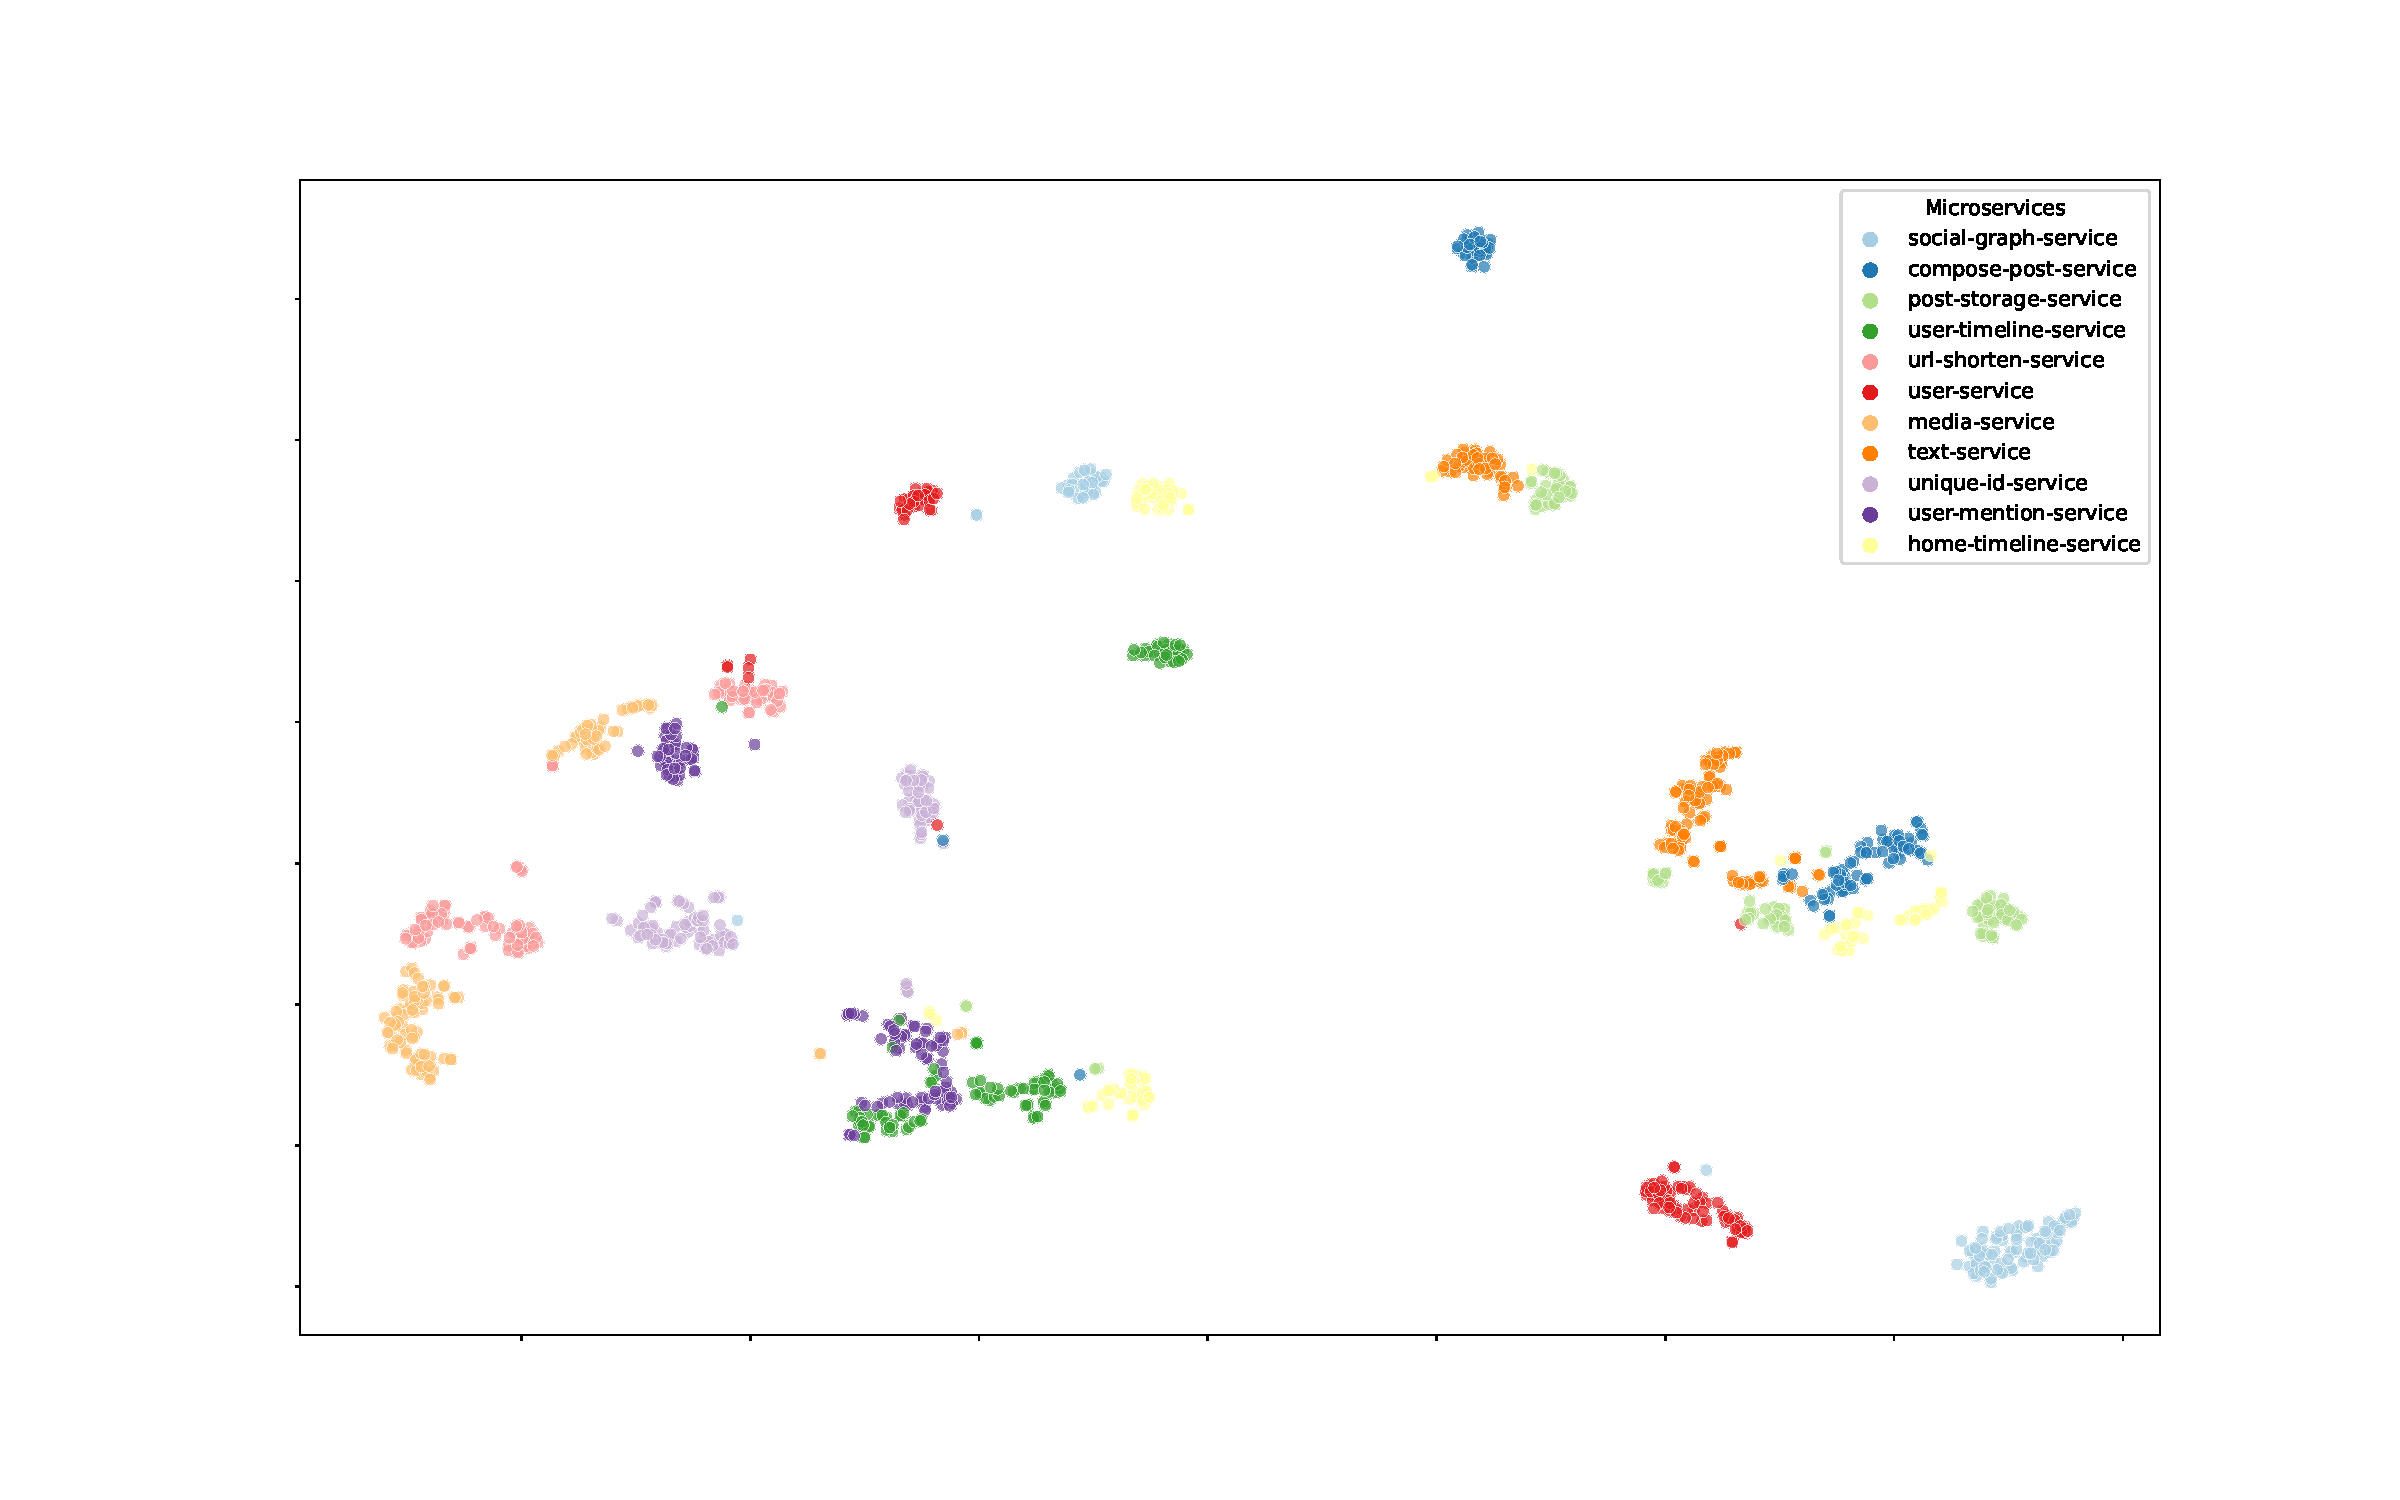
\includegraphics[width=0.95\linewidth]{figures/b.pdf}
\end{minipage}
}
\subfigure[{\name w/o $\mathcal{L}$}]{
\begin{minipage}{0.49\textwidth}
\centering 
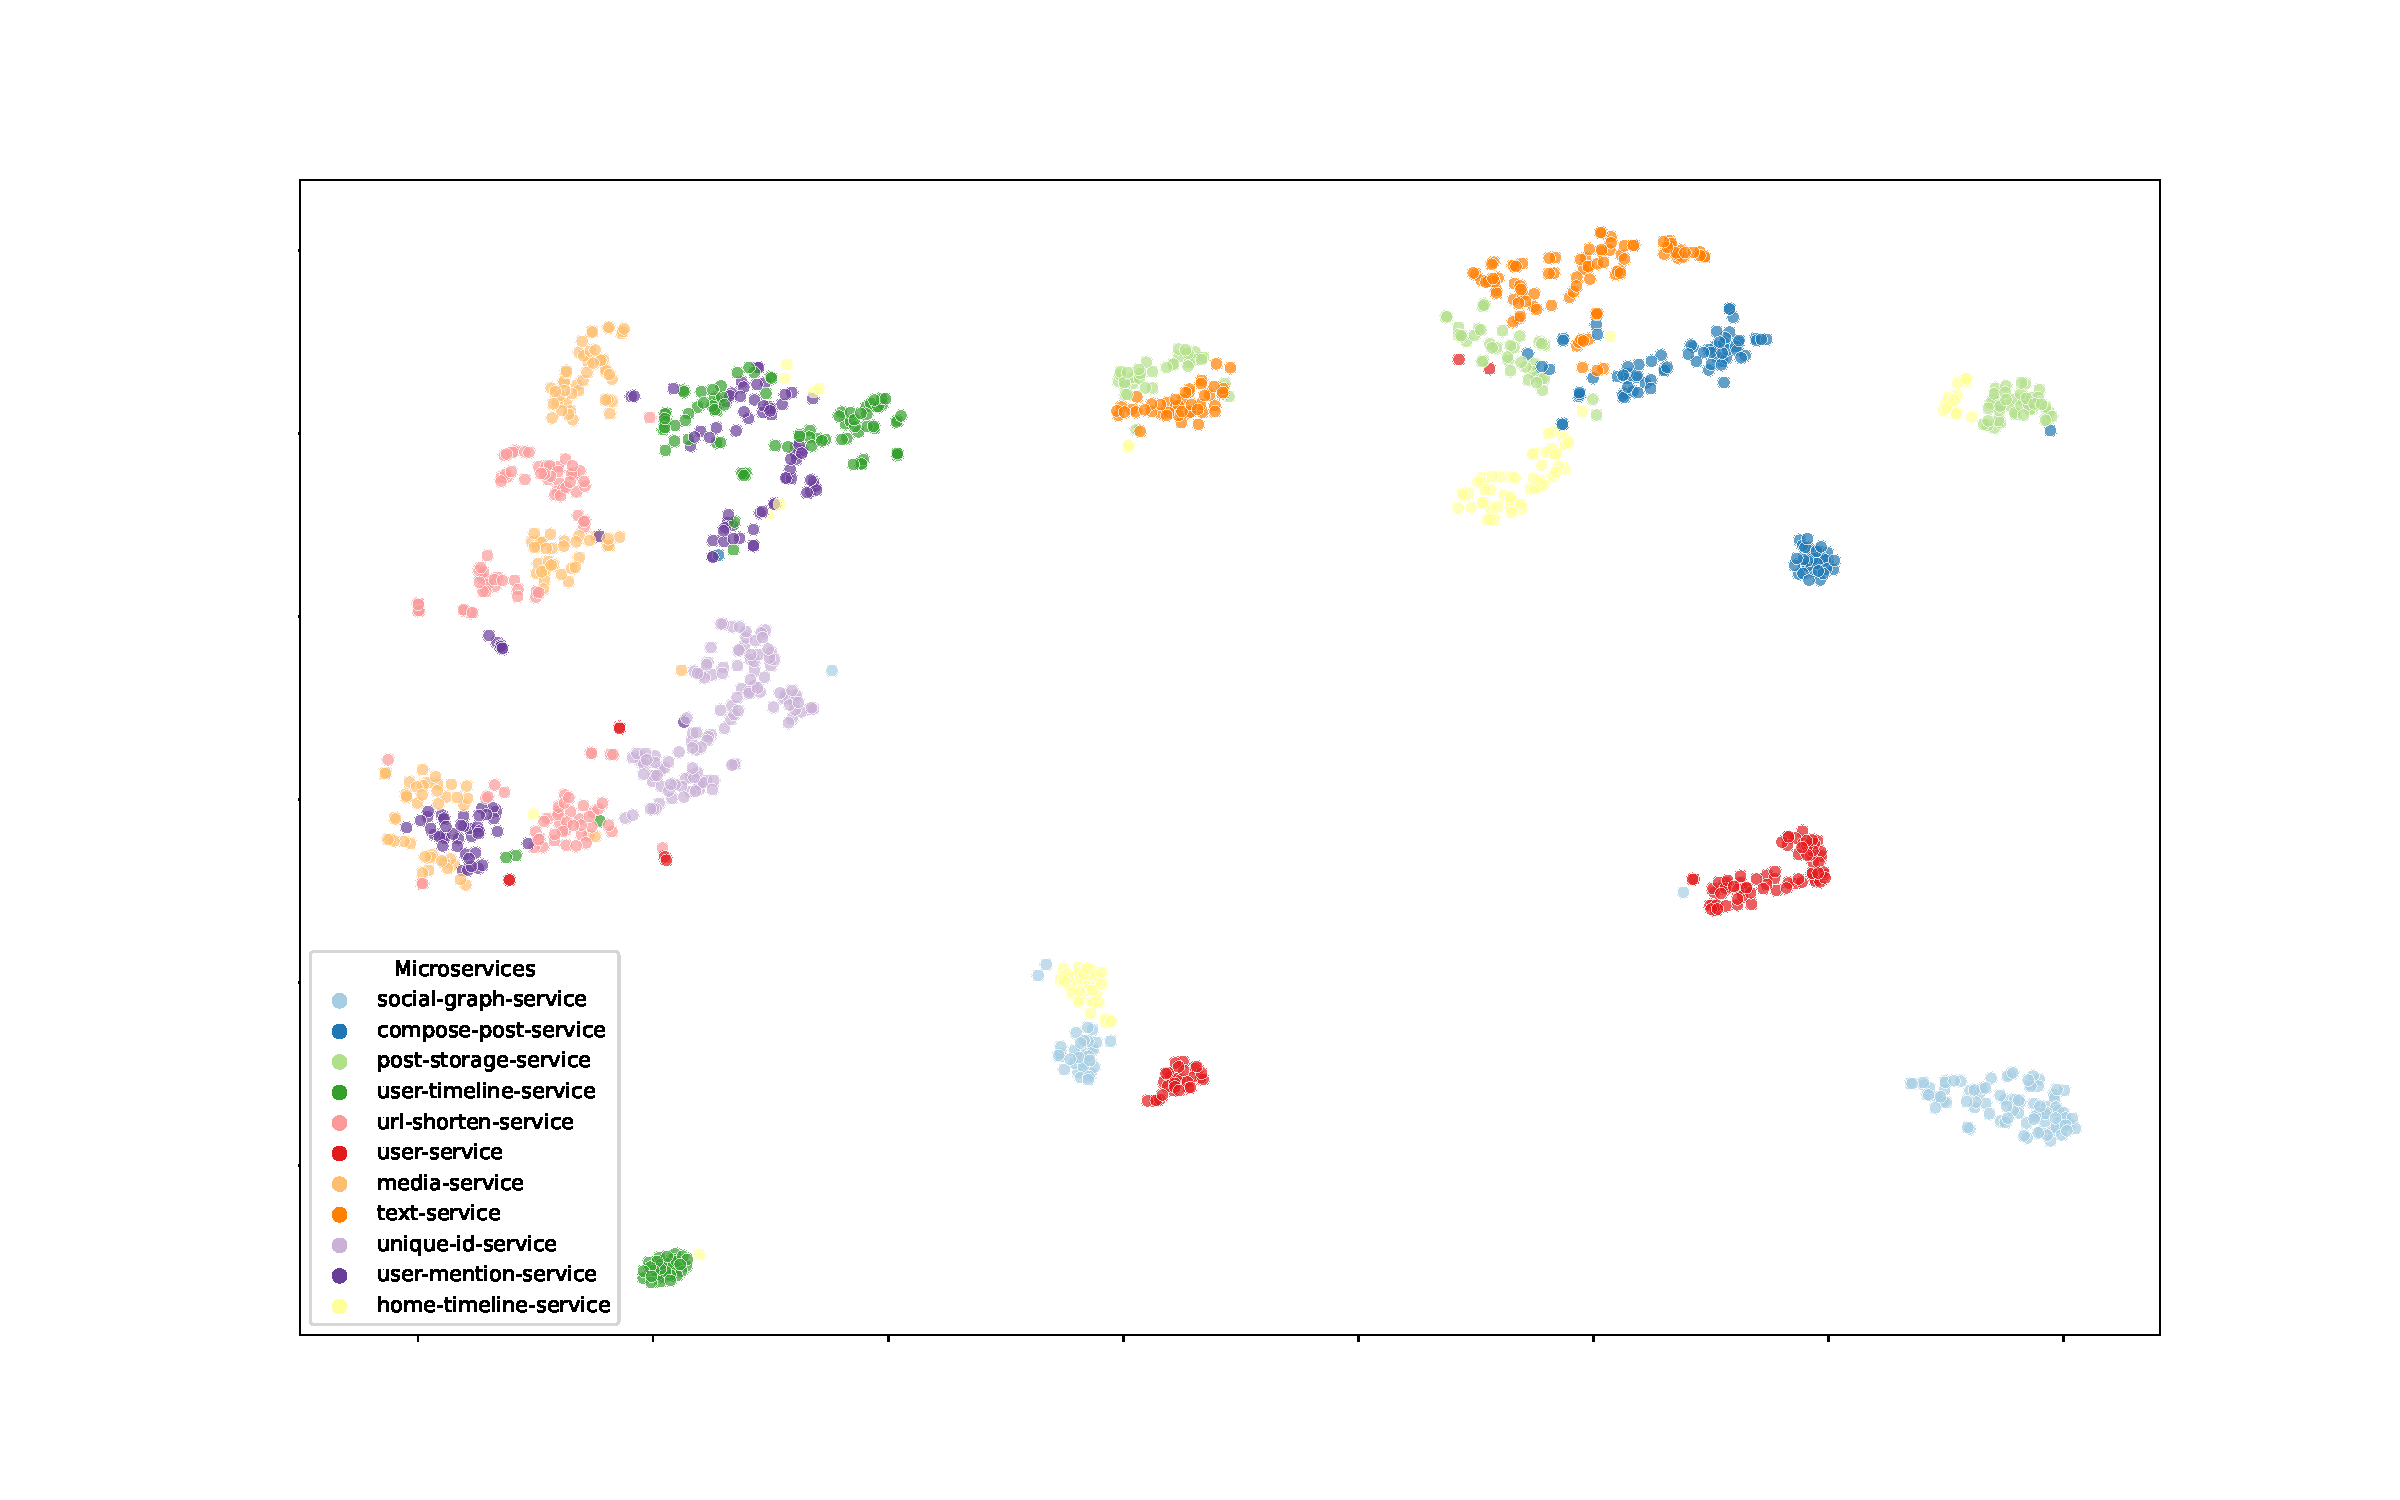
\includegraphics[width=0.95\linewidth]{figures/b-drop-log.pdf}
\end{minipage}
}
\subfigure[{\name w/o $\mathcal{M}$}]{ 
\begin{minipage}{0.49\textwidth}
\centering
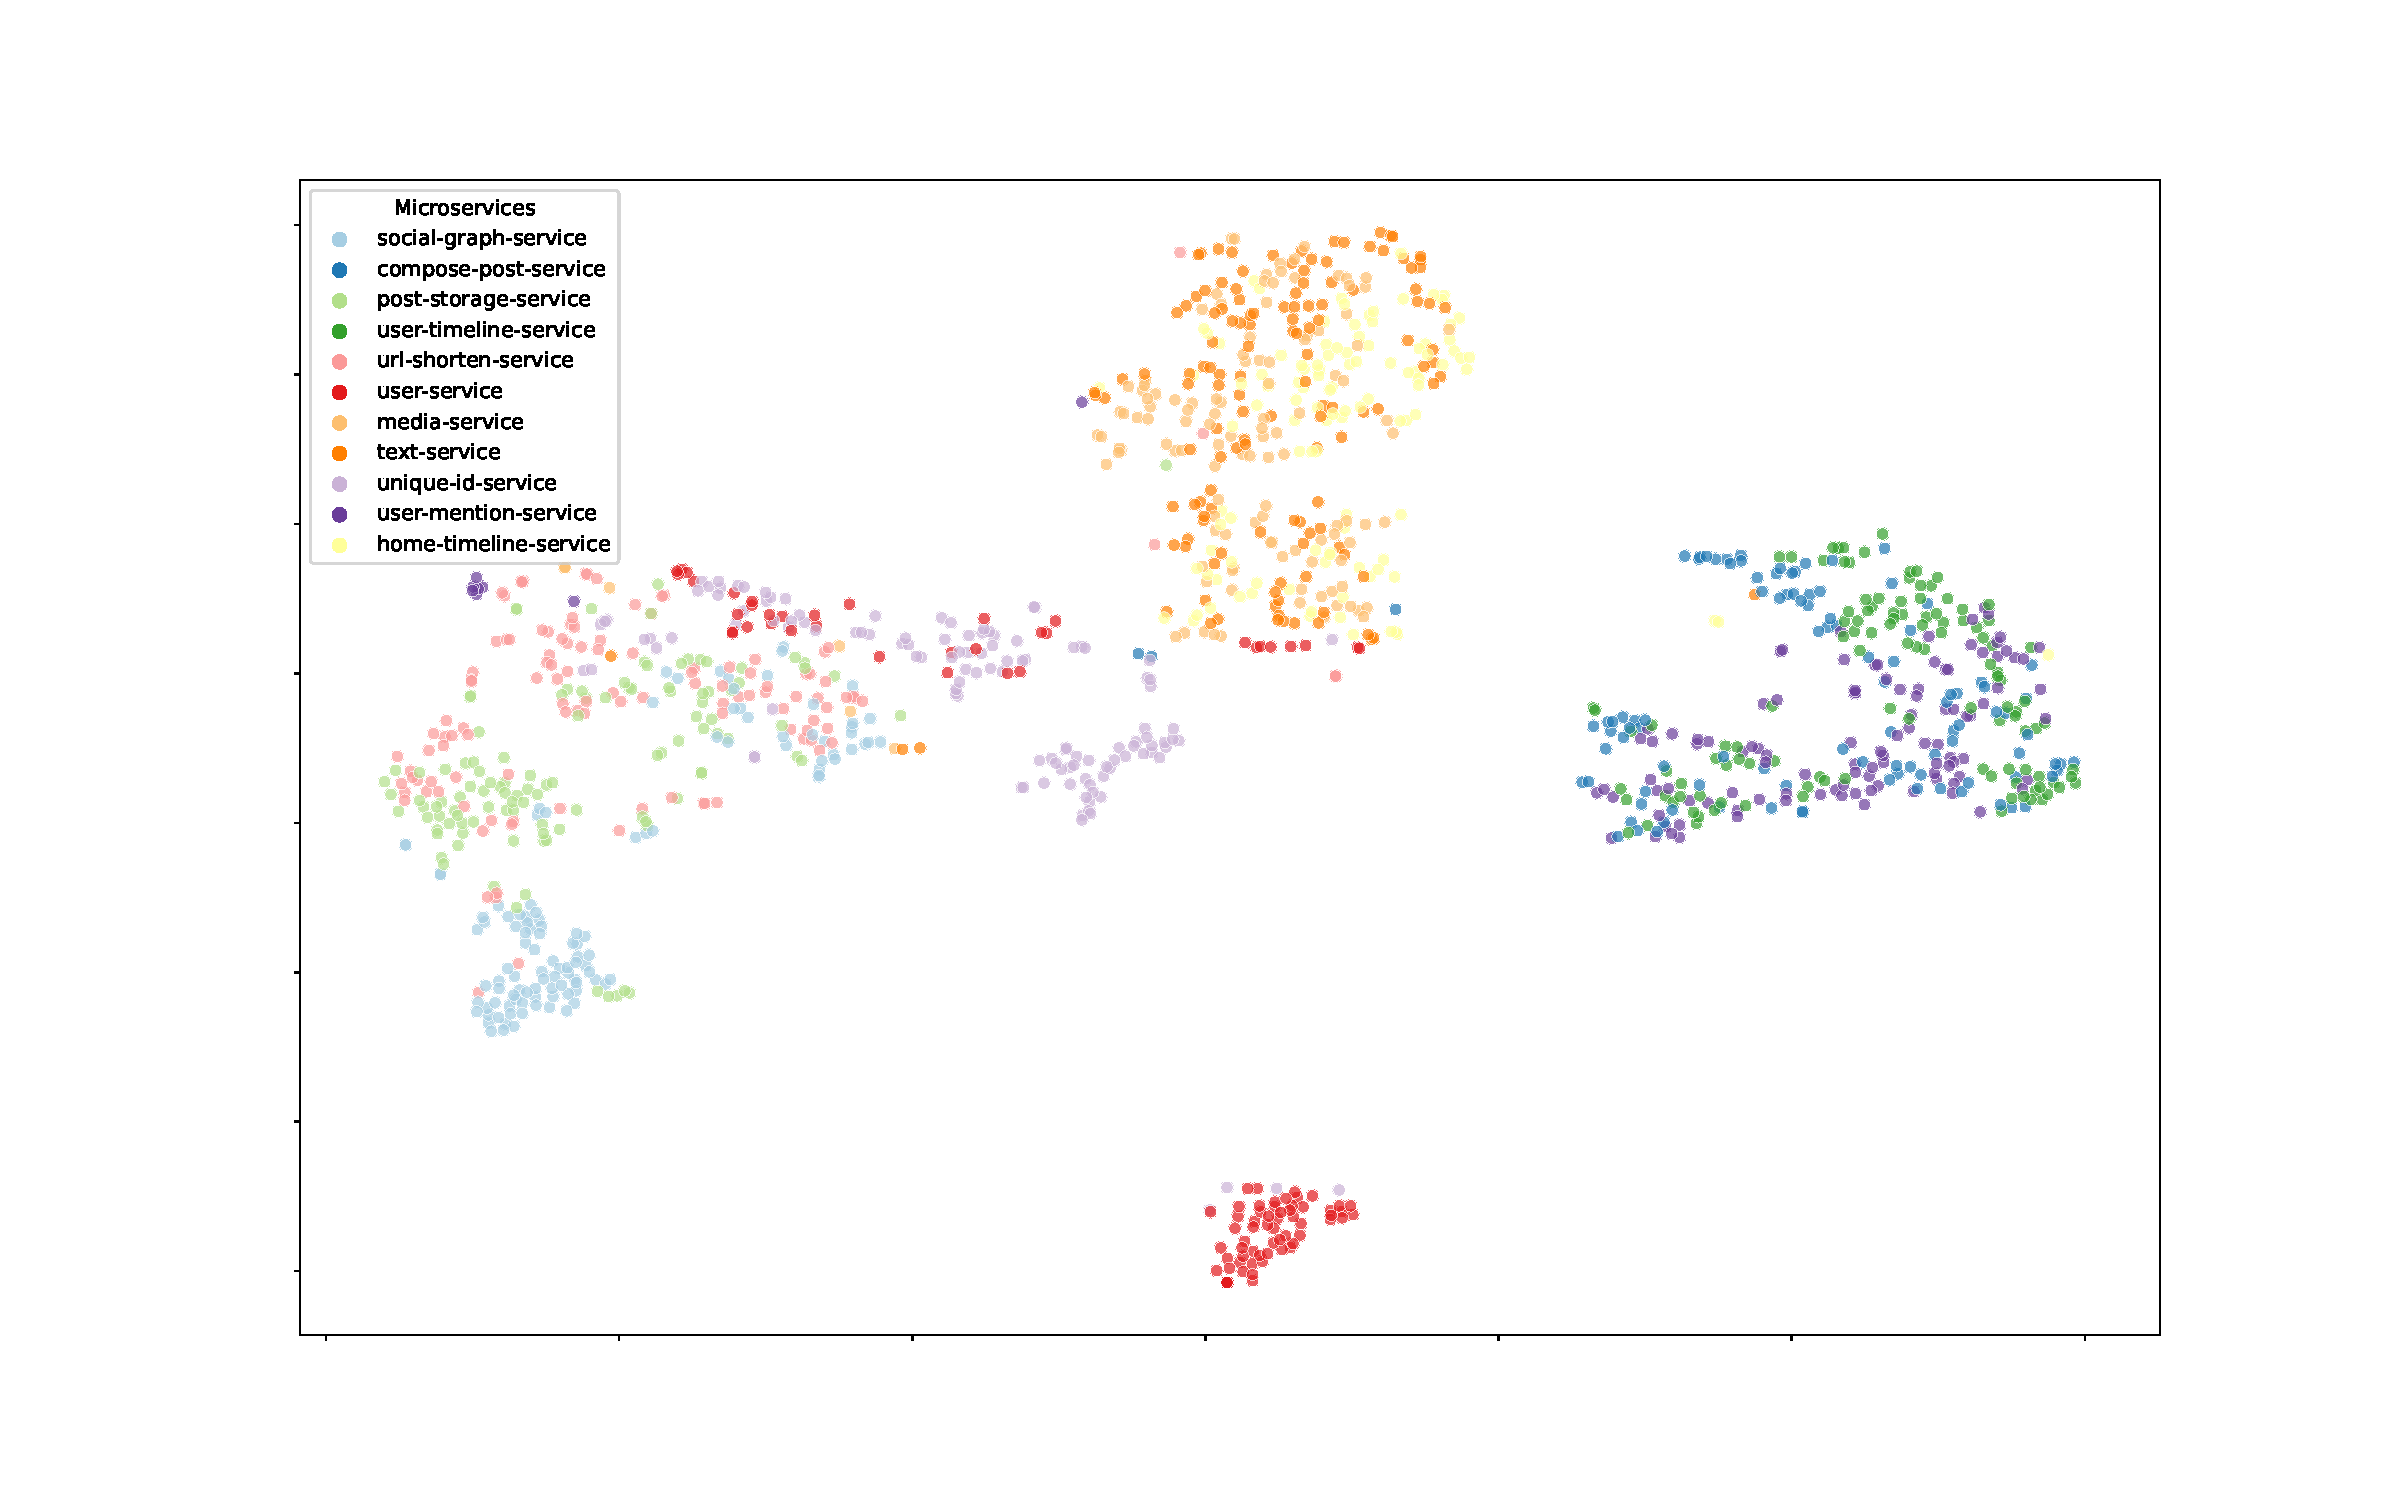
\includegraphics[width=0.95\linewidth]{figures/b-drop-kpi.pdf}
\end{minipage}
}
\vspace{-0.1in}
\caption{Distributions of representations learned by \name and its variants.}
\vspace{-0.3in}
\label{fig:t-sne}
\end{figure}

We can see that the representations learned by \name are the most discriminative, and those learned by {\name~w/o~$\mathcal{L}$} are second-best, while those learned by {\name~w/o~$\mathcal{M}$} are the worst. 
Specifically, \name distributes representations corresponding to the different root causes into different clusters distant from each other in the hyperspace.
In contrast, {\name~w/o~$\mathcal{M}$} learns representations close in space, making it difficult to distinguish them for triage. That is why {\name~w/o~$\mathcal{M}$} delivers poorer performance in localization than \name. The visualization intuitively helps us grasp the usefulness of KPIs in helping pinpoint the root cause.
The discriminativeness of the representations learned by {\name~w/o~$\mathcal{L}$} is in-between, where some clusters are pure while others seem to be a mixture of representations corresponding to different root causes, in line with the experiment results.
We can attribute part of the success of \name to incorporating KPIs and logs, which encourages more discriminative representations of the microservice status with extra clues.

In conclusion, the involved data sources can all contribute to the effectiveness of \name to some degree, and traces contribute the most to the overall effectiveness. This emphasizes the insights about appropriately modeling multi-source data to troubleshoot microservices effectively.

